\documentclass[aspectratio=169,english]{beamer}
\usepackage{siunitx}
\usepackage{physics}
\usepackage{csquotes}
\usepackage{xcolor}
\usepackage{tabularx}

% Document metadata
\title{Surrogates}
\subtitle{Monte Carlo Simulations, Null Hypothesis Testing and Constrained Realizations}
\author[LG]{Luca Gawalleck}
\institute{University Bonn}
\date{19.12.2022}
%\addgraphicspath{{\figs}}

% Image for the title page (use includegraphics option to properly size/place it)
\titlegraphic{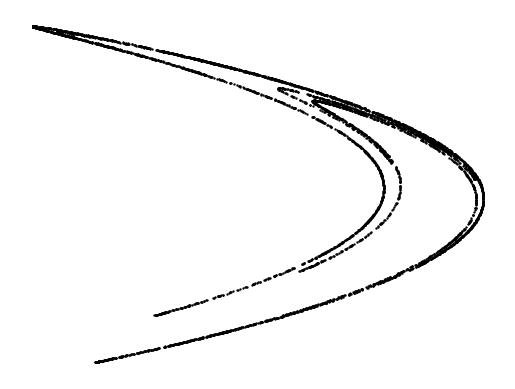
\includegraphics[height=0.8\paperheight]{figs/henon.png}}

\usetheme[sectionstyle=style2]{trigon}

% Define logos to use (comment if no logo)
%\biglogo{trigon_full.pdf} % Used on titlepage only
%\smalllogo{trigon_small.pdf} % Used on top right corner of regular frames

% ------ If you want to change the theme default colors, do it here ------
%\definecolor{tPrim}{HTML}{00843B}   % Green
%\definecolor{tSec}{HTML}{289B38}    % Green light
%\definecolor{tAccent}{HTML}{F07F3C} % Orange

% ------ Packages and definitions used for this demo. Can be removed ------
\usepackage{appendixnumberbeamer} % To use \appendix command
\pdfstringdefDisableCommands{% Fix hyperref translate warning with \appendix
\def\translate#1{#1}%
}
\usepackage{pgf-pie} % For pie charts
\usepackage{caption} % For subfigures
\usepackage{subcaption} % For subfigures
\usepackage{xspace}
\newcommand{\themename}{\textbf{\textsc{trigon}}\xspace}
\usepackage[scale=2]{ccicons} % Icons for CC-BY-SA
\usepackage{booktabs} % Better tables

%==============================================================================
%                               BEGIN DOCUMENT
%==============================================================================
\begin{document}

%--------------------------------------
% Create title frame
\titleframe

%--------------------------------------
% Table of contents
\begin{frame}[shrink=25]{Overview}
  \setbeamertemplate{section in toc}[sections numbered]
  \tableofcontents[hideallsubsections]
\end{frame}

\AtBeginSection{}
%==============================================
\section{Introduction}
%==============================================
\subsection{Different Time Series}
\begin{frame}
    \frametitle{\insertsectionhead}
\framesubtitle{\insertsubsectionhead}
\begin{figure}
    \centering
    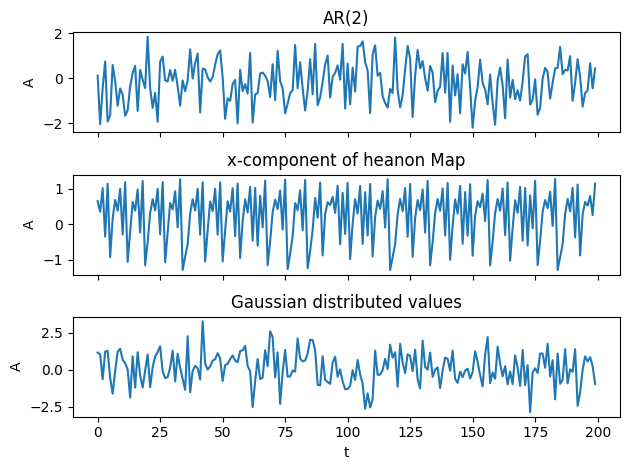
\includegraphics[height=0.8\textheight]{figs/time_series.png}
\end{figure}

\end{frame}

\section{Hypothesis Testing}
\subsection{$H_0$ and $H_1$}
\begin{frame}
  \frametitle{\insertsectionhead}
\framesubtitle{\insertsubsectionhead}
\begin{columns}
  \begin{column}{0.5\textwidth}
  \centering
  \begin{figure}
      \centering
      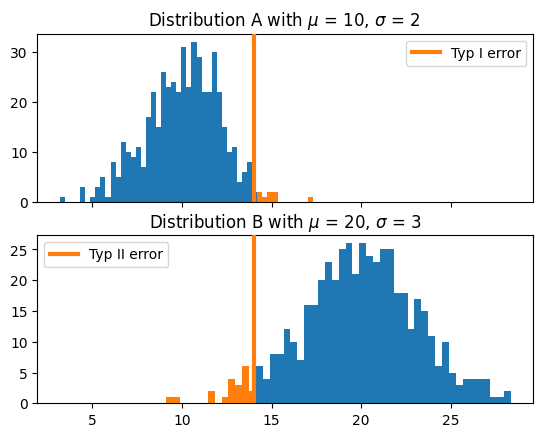
\includegraphics[width=0.9\textwidth]{figs/hypothesis.png}
  \end{figure}
  \end{column}
  \begin{column}{0.5\textwidth}
  \centering
  \begin{itemize}
    \item asking yes or no question
    \item accept or reject the Hypothesis
    \item discriminating statistics $T$
  \end{itemize}
  \begin{table}[]
    \centering
    \begin{tabular}{lllll}
                 & $H_0$                   & $H_1$                   &  &  \\
    Result $H_0$ & correct                 & Type II error ($\beta$) &  &  \\
    Result $H_1$ & Type I error ($\alpha$) & correct                 &  &  
    \end{tabular}
    \end{table}
    \begin{itemize}
      \item $\alpha$: \textit{size}
      \item $1-\beta$: \textit{power}
      \item one and two sided tests
    \end{itemize}
  \end{column}
  \end{columns}
\end{frame}
\subsection{simple and composite}
\begin{frame}
\frametitle{\insertsectionhead}
\framesubtitle{\insertsubsectionhead}
let $\mathcal{F}$ be the space of all processes under consideration and $\mathcal{F}_\phi\subset \mathcal{F}$ the processes which are consistent with the null hypothesis. According to the Null Hypothesis the process $F$ that generated the data, is an element of $\mathcal{F}_\phi$. If $\mathcal{F}_\phi$ consists just a single member, the Null Hypothesis is \textit{single} otherwise it is \textit{composite} \cite{THEILER1996221}
\end{frame}

\section{Surrogates}
\subsection{typical realization}
\begin{frame}
  \frametitle{\insertsectionhead}
  \framesubtitle{\insertsubsectionhead}
  fit a model like
  \begin{description}
    \item[autoregressive (AR):] $\vec{x}_{n+1} = \sum_{i=0}^{p-1} A^i \vec{x}_{n-i} + \mathrm{noise}$
    \item[Hénon map:] $ \vec{x}_{n+1} = \begin{cases} x_{n+1} = 1 - a x_n^2+y_n\\ y_{n+1} = b x_n \end{cases}$
  \end{description}
  \begin{itemize}
    \item Confidence interval $95\,\%$ ($\alpha=0.05$)
    \item $T$ must be \textit{pivotal} ($T$ is the same $\forall F \in \mathcal{F}_\phi)$ if NH is composite
    \item often only in limit $n\to\infty$
  \end{itemize}
\end{frame}

\subsection{Monte Carlo Simulation}
\begin{frame}
  \frametitle{\insertsectionhead}
  \framesubtitle{\insertsubsectionhead}
\begin{itemize}
  \item Generating random variables according to a distribution
  \item Use these variables to simulate an experiment 
  \item possible with any distribution with MC 
  \item Bootstraps $\rightarrow$ measuring error bars 
  \item Testing Null Hypothesis
\end{itemize}
\end{frame}


\subsection{constrained realizations}
\begin{frame}
  \frametitle{\insertsectionhead}
  \framesubtitle{\insertsubsectionhead}
\begin{itemize}
  \item random samples with constraints
  \item useful if $T$ or the model is unknown 
\end{itemize}
\subsection{Number of Surrogates}
Number of Surrogates
\begin{itemize}
  \item upper limit $\rightarrow$ often not infinit possibilities
  \item minimal number through convergence of the distribution
\end{itemize}
\begin{gather}
  M = \frac{K}{\alpha}-1
\end{gather}
with $K$ is 1 for one sided test and 2 for two sided test \cite{LANCASTER20181}
\end{frame}

\section{Testing for IID data}
\begin{frame}
  \frametitle{\insertsectionhead}
  \framesubtitle{\insertsubsectionhead}
\begin{itemize}
  \item \textbf{Null Hypothesis} the data are independent and identically distributed
  \item randomly shuffle the values of the time series
\end{itemize}
discriminating statistic
\begin{gather*}
  T = A(1) = \frac{1}{n-1} \sum_{i=0}^{n}(x(i)-\overline{x})\frac{(x(i+1)-\overline{x})}{\overline{(x-\overline{x})^2}} \quad \text{with} \quad \overline{(x-\overline{x})^2} = \sqrt{\frac{1}{n}\sum_{i=0}^n (x(i)-\overline{x})^2}
\end{gather*}
\end{frame}


\subsection{AR2}
\begin{frame}
  \frametitle{\insertsectionhead}
  \framesubtitle{\insertsubsectionhead}
\begin{figure}
  \centering
  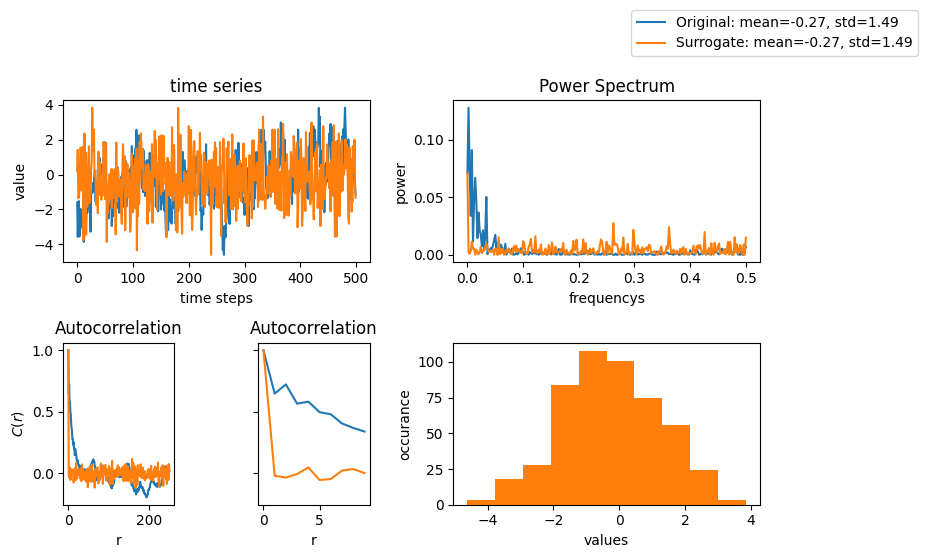
\includegraphics[height=0.8\textheight]{figs/IID_ar2.png}
\end{figure}
\end{frame}

\subsection{x-component Hénon}
\begin{frame}
  \frametitle{\insertsectionhead}
  \framesubtitle{\insertsubsectionhead}
\begin{figure}
  \centering
  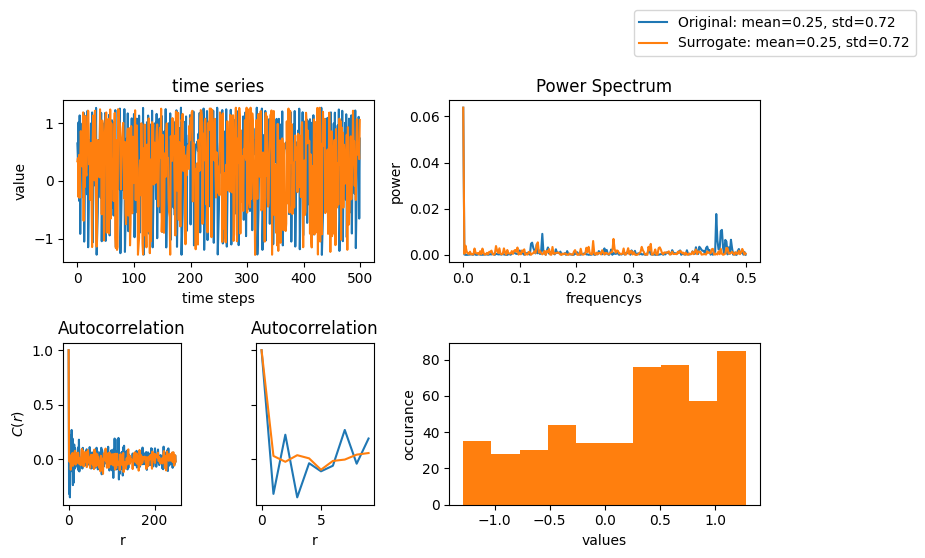
\includegraphics[height=0.8\textheight]{figs/IID_henon.png}
\end{figure}
\end{frame}

\subsection{discriminating statistics}
\begin{frame}
  \frametitle{\insertsectionhead}
  \framesubtitle{\insertsubsectionhead}
\begin{figure}
  \centering
  \begin{subfigure}[b]{0.4\textwidth}
    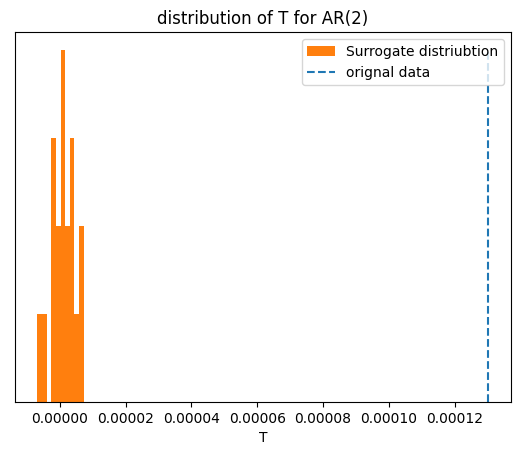
\includegraphics[width=\textwidth]{figs/IID_ar2_T.png}
  \end{subfigure}
  \begin{subfigure}[b]{0.4\textwidth}
    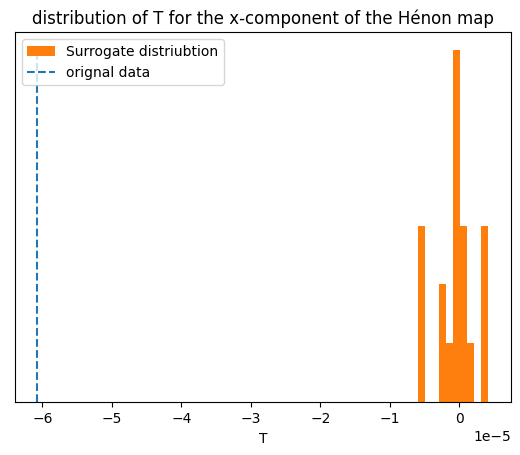
\includegraphics[width=\textwidth]{figs/IID_henon_T.png}
  \end{subfigure}
\end{figure}
\end{frame}

\section{Testing for Nonlinearity}
\begin{frame}
  \frametitle{\insertsectionhead}
  \framesubtitle{\insertsubsectionhead}
  \begin{itemize}
    \item \textbf{Null Hypothesis} Data generated by linear stationary process probably with noise and can be fully characterized by linear statistics i.e. \textit{mean}, \textit{standard deviation} and \textit{autocorrelation}. \cite{LANCASTER20181}
    \item non stationary possible
  \end{itemize}
  Wiener-Khinchin-theorem
  \begin{gather*}
    S(f) = \int_{-\infty}^{\infty}A(\tau) \mathrm{e}^{-i 2\pi f \tau}\mathrm{d}\tau
  \end{gather*}
\end{frame}

\subsection{Prepocessing}
\begin{frame}
  \frametitle{\insertsectionhead}
  \framesubtitle{\insertsubsectionhead}
  \begin{itemize}
    \item removing trends that are not important
    \item subtract the mean
    \item end-to-end mismatch
    \begin{itemize}
      \item periodic boundary conditions
      \item a missmatch is a $\theta$-function 
      \item window functions not linear 
      \item truncate the timeseries
    \end{itemize}
  \end{itemize}
\end{frame}

\subsection{FT-Surrogate}
\begin{frame}
  \frametitle{\insertsectionhead}
  \framesubtitle{\insertsubsectionhead}
  \begin{itemize}
    \item FFT
    \item random phases $\phi$ s.t. $\phi(f)=-\phi(-f)$ 
    \item IFFT
  \end{itemize}
\end{frame}

\begin{frame}
  \frametitle{\insertsectionhead}
  \framesubtitle{\insertsubsectionhead}
\begin{figure}
  \centering
  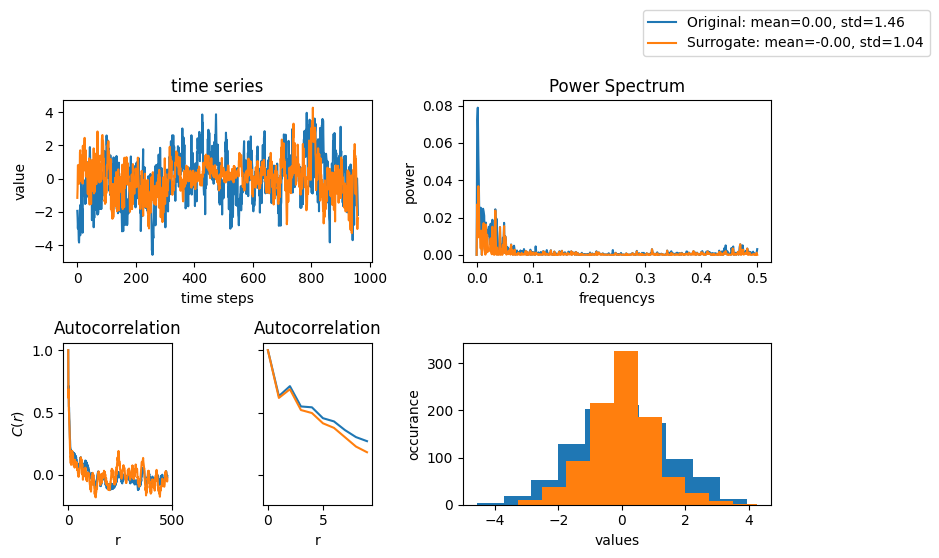
\includegraphics[height=0.8\textheight]{figs/FT.png}
\end{figure}
\end{frame}

\subsection{AAFT-Surrogates}
\begin{frame}
  \frametitle{\insertsectionhead}
  \framesubtitle{\insertsubsectionhead}
  \begin{itemize}
    \item rescale values to be Gaussian
    \item apply FT 
    \item rescale back to have same amplitude distribution
  \end{itemize}
\end{frame}

\begin{frame}
  \frametitle{\insertsectionhead}
  \framesubtitle{\insertsubsectionhead}
\begin{figure}
  \centering
  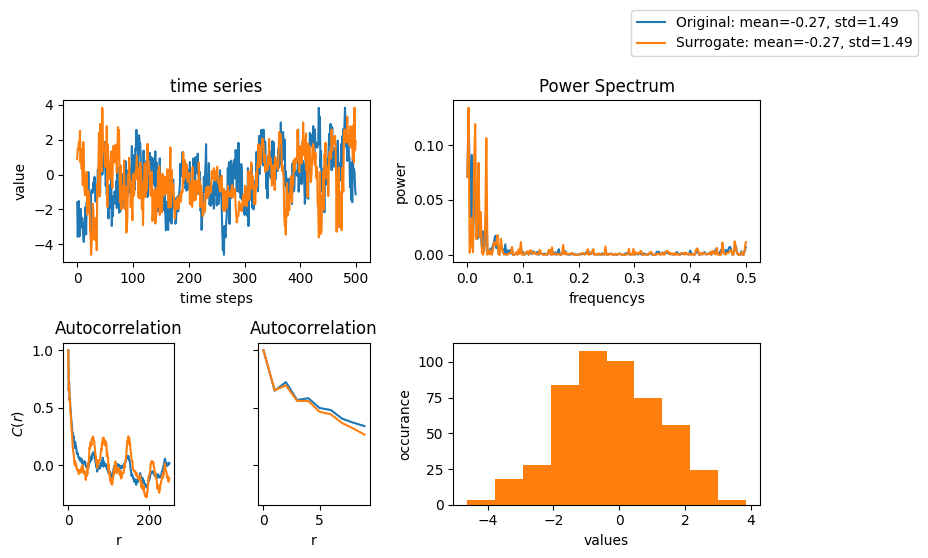
\includegraphics[height=0.8\textheight]{figs/AAFT.png}
\end{figure}
\end{frame}

\subsection{IAAFT-Surrogates}
\begin{frame}
  \frametitle{\insertsectionhead}
  \framesubtitle{\insertsubsectionhead}
  \begin{itemize}
    \item iterate since convergence criteria AAFT
    \item better match for autocorrelation and power spectrum
  \end{itemize}
\end{frame}

\begin{frame}
  \frametitle{\insertsectionhead}
  \framesubtitle{\insertsubsectionhead}
\begin{figure}
  \centering
  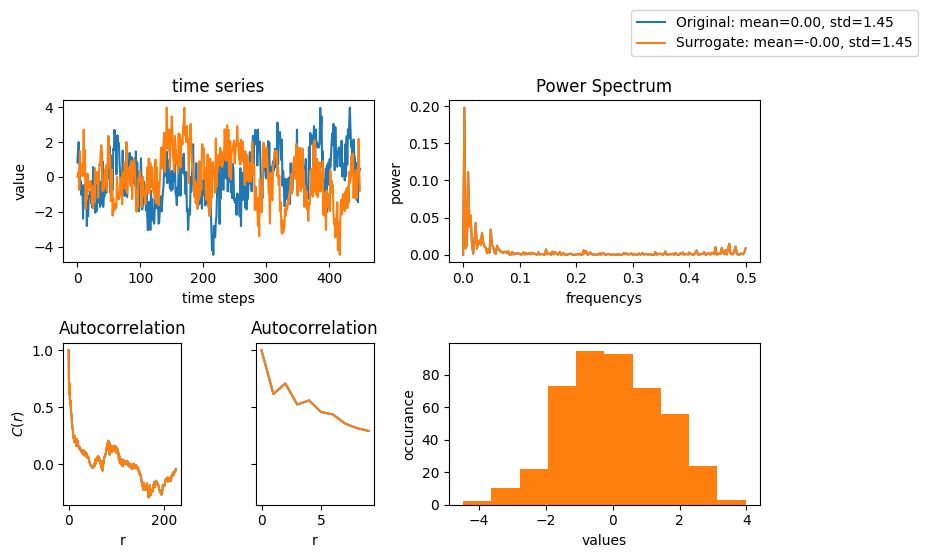
\includegraphics[height=0.8\textheight]{figs/IAAFT.png}
\end{figure}
\end{frame}

\subsection{Discriminating Statistics}
\begin{frame}
  \frametitle{\insertsectionhead}
  \framesubtitle{\insertsubsectionhead}
\subsection{discriminating statistics}
\begin{gather*}
  T = \frac{\langle(x(i+1)-x(i))^3 \rangle}{\langle (x(i+1)-x(i))^2 \rangle^{3/2} } + 20A(1)
\end{gather*} \cite{THEILER1996221}
\begin{figure}
  \centering
  \begin{subfigure}[b]{0.3\textwidth}
    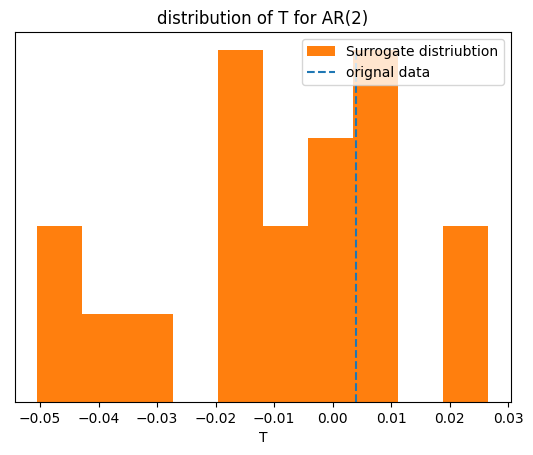
\includegraphics[width=\textwidth]{figs/non_lin_ar2_T.png}
  \end{subfigure}
  \begin{subfigure}[b]{0.3\textwidth}
    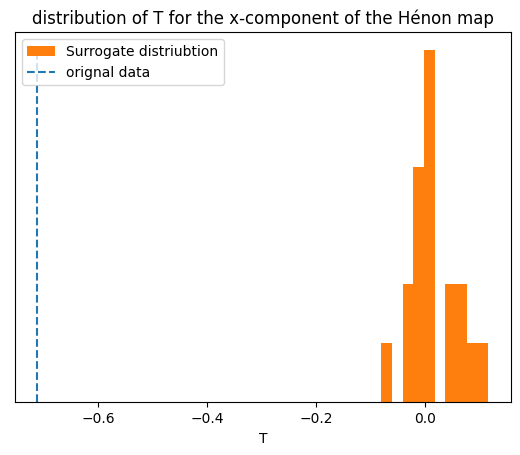
\includegraphics[width=\textwidth]{figs/non_lin_henon_T.png}
  \end{subfigure}
\end{figure}
\end{frame}

\section{Delay-Coordinate Embedding}
\begin{frame}
  \frametitle{\insertsectionhead}
  \framesubtitle{\insertsubsectionhead}
  reconstruct $m$-dimensional phase space with $x(t), x(t-\tau), x(t-2\tau), \ldots$ as axes
  \begin{itemize}
    \item \textbf{Takens's Theorem}: for right $\tau$ and enough dimensions $m$ the embedded dynamics has the same topology as the original state-space of the system
  \end{itemize}
\end{frame}

\subsection{Correlation Dimension}
\begin{frame}
  \frametitle{\insertsectionhead}
  \framesubtitle{\insertsubsectionhead}

\begin{description}
  \item[pointwise dimension] 

  $d_\mathrm{p}$: number of points $N_x(\varepsilon)$ within $\varepsilon$ around a point $x$
\begin{gather*}
N_x(\varepsilon) \propto \varepsilon^{d_\mathrm{p}}
\end{gather*}
\item[correlation dimension]
$d_\mathrm{corr}$: average $N_x(\varepsilon)$ over lots of $x$: $N_x(\varepsilon)\to C(\varepsilon)$

\begin{gather*}
C(\epsilon) \propto \varepsilon^{d_\text{corr}}\\
C(\varepsilon) =\frac{1}{N(N-1)} \sum_{i=1}^N\sum_{j=i+1}^N \Theta(\varepsilon-||x_i-x_j||)\\
\end{gather*}

\end{description}
\end{frame}

\subsection{measurement of $d_\mathrm{corr}$ for x-component of the Hénon Map}
\begin{frame}
  \frametitle{\insertsectionhead}
  \framesubtitle{\insertsubsectionhead}
  \begin{figure}
    \centering
    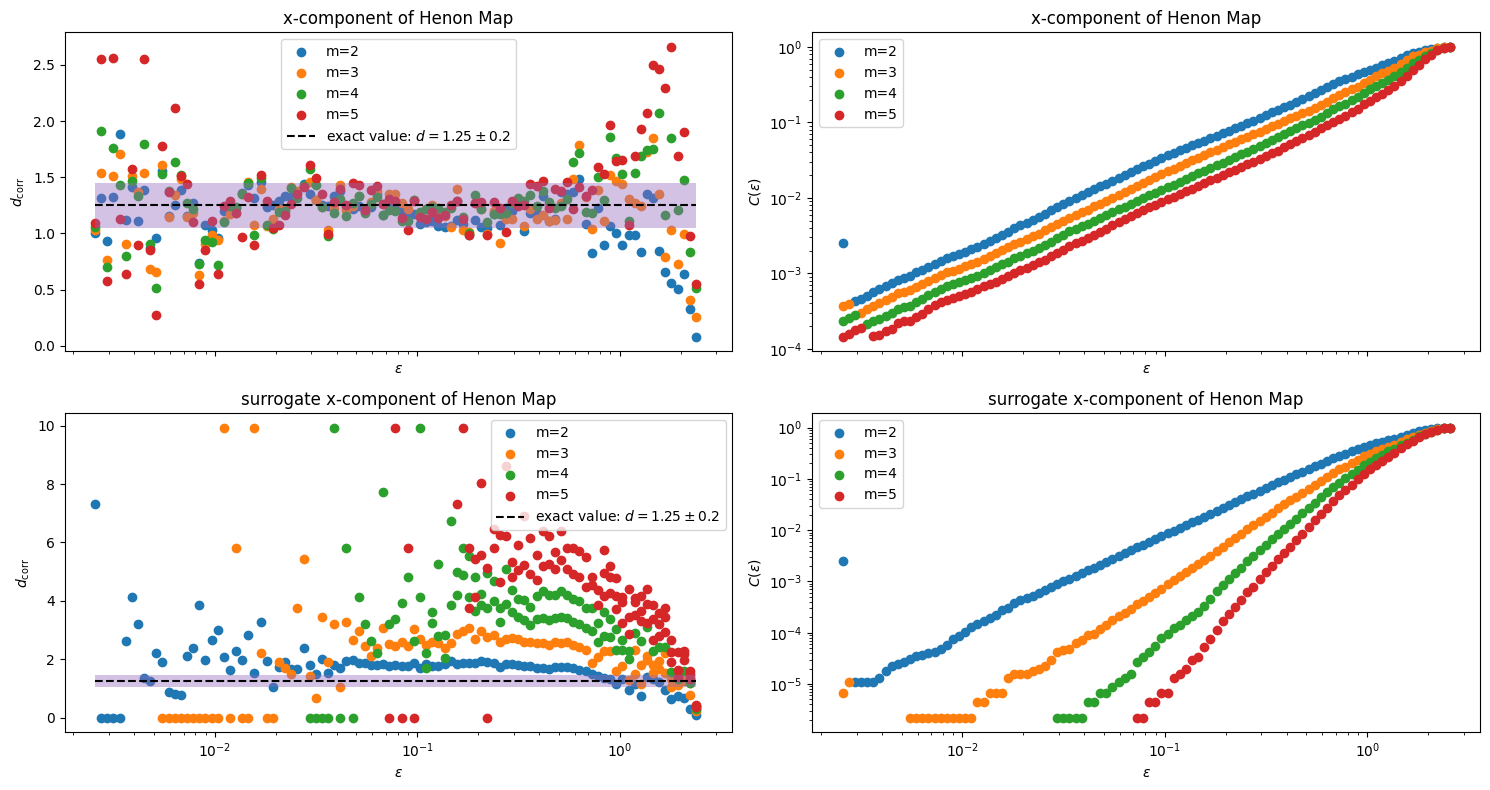
\includegraphics[height=0.8\textheight]{figs/d_henon.png}
  \end{figure}
\end{frame}

\subsection{measurement of $d_\mathrm{corr}$ for AR(2)}
\begin{frame}
  \frametitle{\insertsectionhead}
  \framesubtitle{\insertsubsectionhead}
  \begin{figure}
    \centering
    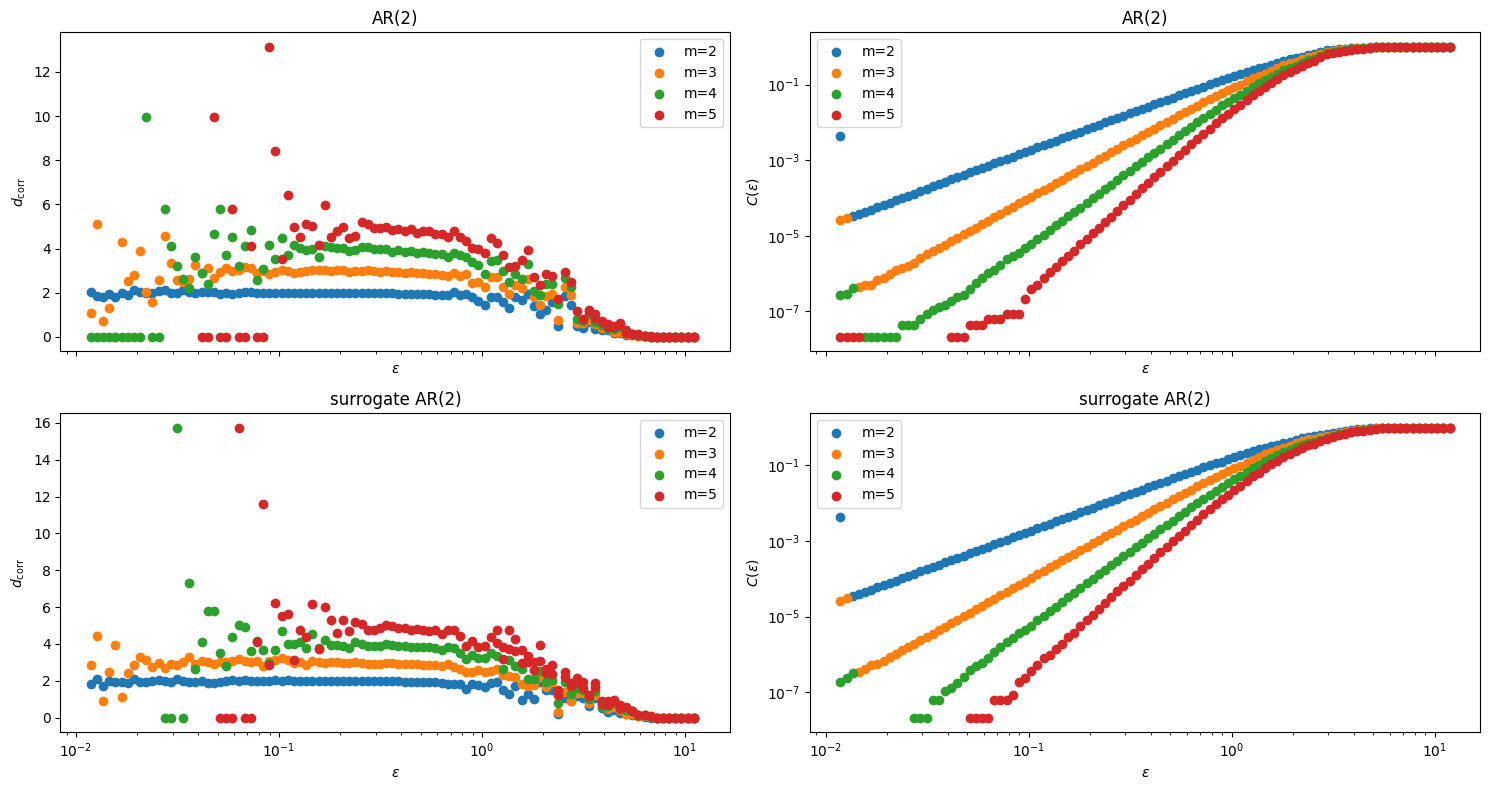
\includegraphics[height=0.8\textheight]{figs/d_ar2.png}
  \end{figure}
\end{frame}

\section{EEG}
\begin{frame}
  \frametitle{\insertsectionhead}
  \framesubtitle{\insertsubsectionhead}
  \begin{figure}
    \centering
    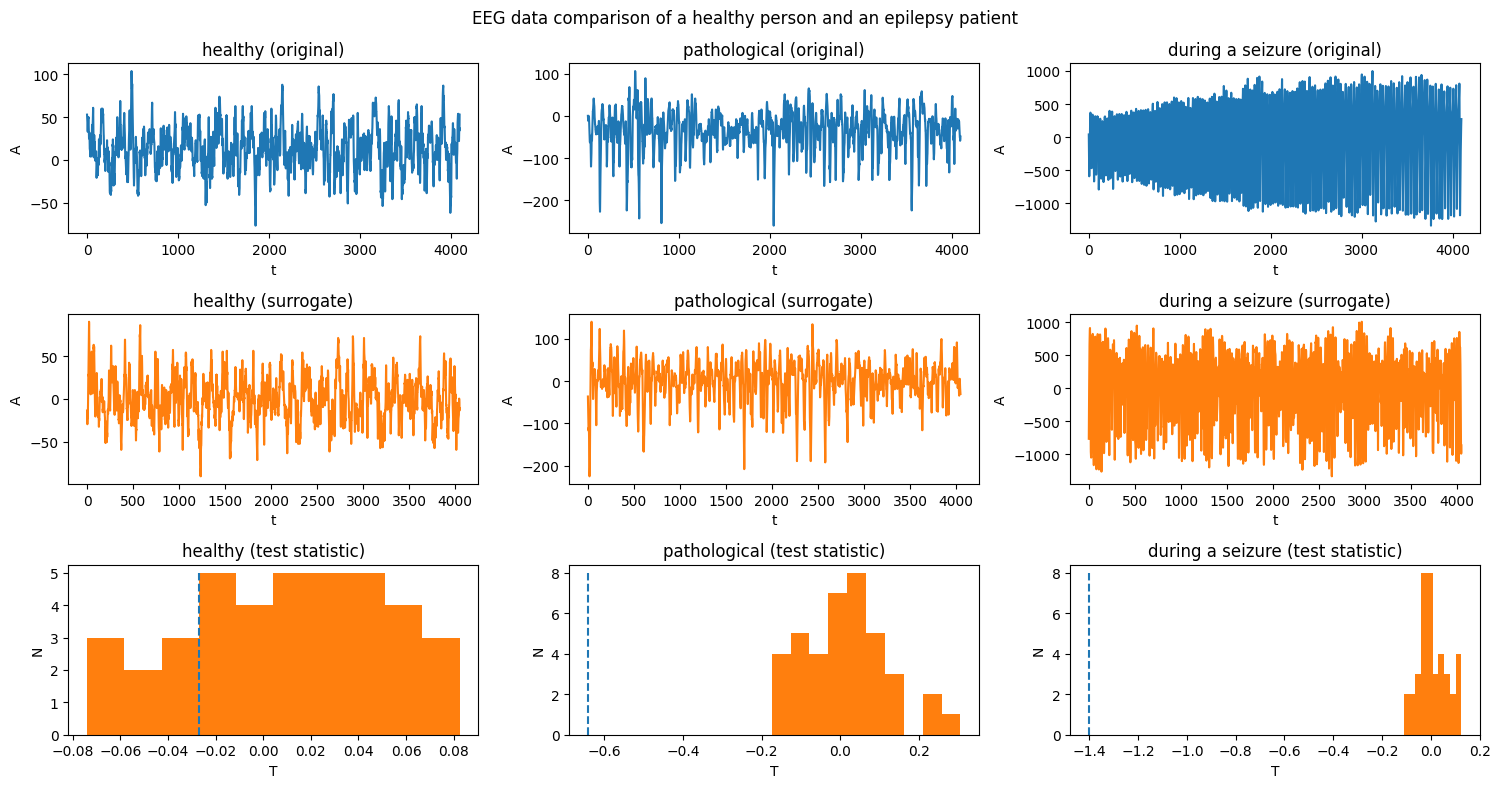
\includegraphics[height=0.8\textheight]{figs/EEG.png}
  \end{figure}
\end{frame}


\begin{frame}{Conclusion}
  \begin{itemize}
    \item possibility for simulate data without knowledge of distribution through Monte Carlo Simulation
    \item non linearity not clearly measurable but evidences can be found
    \item anomalies in e.g. EEG Data can be found 
  \end{itemize}
\end{frame}

\appendix

\begin{frame}[shrink=25]{References}
  % Bildquelle: \nocite{DWave_doc}
  \nocite{Theiler1992TestingFN}
  \bibliography{demo}
  \bibliographystyle{abbrv}
  \nocite{Kugiumtzis1999-qt}
\end{frame}


\end{document}
